
\begin{enumerate}
    \item A conducting loop in the shape of a right angled isosceles triangle of height 10 cm is kept such that the 90° vertex is very close to an infinitely long conducting wire (see the figure). The wire is electrically insulated from the loop. The hypotenuse of the triangle is parallel to the wire. The current in the triangular loop is in counterclockwise direction and increased at a constant rate of \(10\ As^{-1}\). Which of the following statement(s) is(are) true?
        \begin{tasks}(1)
            \task The magnitude of induced \emph{emf} in the wire is \(\left(\frac{\mu_0}{\pi}\right)\) volt
            \task If the loop is rotated at a constant angular speed about the wire, an additional \emph{emf} of \(\frac{\mu_0}{\pi}\) volt is induced in the wire
            \task The induced current in the wire is in opposite direction to the current along the hypotenuse
            \task There is a repulsive force between the wire and the loop
        \end{tasks}
\end{enumerate}
\begin{center}
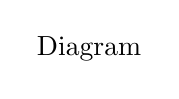
\begin{tikzpicture}
\node {Diagram};
\end{tikzpicture}
\end{center}
